%%%%%%%%%%%%%%%%%%%%%%%%%%% asme2ej.tex %%%%%%%%%%%%%%%%%%%%%%%%%%%%%%%
% Template for producing ASME-format journal articles using LaTeX    %
% Written by   Harry H. Cheng, Professor and Director                %
%              Integration Engineering Laboratory                    %
%              Department of Mechanical and Aeronautical Engineering %
%              University of California                              %
%              Davis, CA 95616                                       %
%              Tel: (530) 752-5020 (office)                          %
%                   (530) 752-1028 (lab)                             %
%              Fax: (530) 752-4158                                   %
%              Email: hhcheng@ucdavis.edu                            %
%              WWW:   http://iel.ucdavis.edu/people/cheng.html       %
%              May 7, 1994                                           %
% Modified: February 16, 2001 by Harry H. Cheng                      %
% Modified: January  01, 2003 by Geoffrey R. Shiflett                %
% Use at your own risk, send complaints to /dev/null                 %
%%%%%%%%%%%%%%%%%%%%%%%%%%%%%%%%%%%%%%%%%%%%%%%%%%%%%%%%%%%%%%%%%%%%%%

%%% use twocolumn and 10pt options with the asme2ej format


\documentclass[twocolumn,10pt]{asme2ej}

\usepackage{amssymb,fleqn,graphicx,ctable,mathptmx,helvet,hyperref,courier,subfigure,multirow,makeidx,graphicx,lscape,morefloats,algorithmic,algorithm,amsmath,balance,placeins,flafter,epsfig,color}
\usepackage[noadjust]{cite}
\usepackage{filecontents}
\usepackage{enumerate}
%\usepackage{enumitem}
\usepackage{titlesec}


\title{Multiple Surrogate Assisted Many-objective Optimization for {\color{blue}Computationally Expensive} Engineering Design}

\author{Kalyan Shankar Bhattacharjee, Hemant Kumar Singh, Tapabrata Ray
	\affiliation{
		School of Engineering and IT, The University of New South Wales, Canberra, Australia\\
		Email: k.bhattacharjee@student.adfa.edu.au, \{h.singh,t.ray\}adfa.edu.au\\
	}	
}



\begin{document}

\maketitle    


%%%%%%%%%%%%%%%%%%%%%%%%%%%%%%%%%%%%%%%%%%%%%%%%%%%%%%%%%%%%%%%%%%%%%%
\begin{abstract}
	{\it Engineering design often involves solutions to problems involving
multiple conflicting performance criteria, commonly
referred to as multi-objective optimization problems~(MOP).
MOPs are known to be particularly challenging if the number
of objectives is more than three. This has motivated recent attempts to solve MOPs with more than
three objectives, which are now more specifically referred to
{\color{blue}as ``many-objective'' optimization problems}~(MaOPs). Evolutionary algorithms used to solve such problems are known to require
evaluation of numerous designs prior to convergence
to near-optimal solutions, which is not practical for engineering applications involving computationally
expensive evaluations such as computational fluid
dynamics, Finite Element Analysis etc. While
the use of surrogates has been a commonly studied for single-objective
optimization, there is scarce literature on their use
for MOPs/MaOPs. This paper attempts
to bridge this research gap by introducing a surrogate assisted
optimization algorithm for solving MOP/MaOP within a limited computing
budget. The algorithm relies on principles of decomposition
and adaption of reference vectors for effective search.
The flexibility of function representation is offered through
the use of multiple types of surrogate models. Furthermore,
to efficiently deal with constrained MaOPs, marginally infeasible
solutions are promoted during initial phases of the
search. The performance of the proposed algorithm bench-marked with state-of-the-art approaches
using a variety of problems for up to 10 objective problems. Thereafter, a
case study involving {\color{blue}vehicle design} is presented
highlighting the competence of the proposed approach.}
\end{abstract}


\section{Introduction}
\label{sec:KHTsec:1}


It is common to come across situations in engineering design where multiple conflicting performance criteria need to be simultaneously optimized~\cite{deb2001multi,Asafuddoula2015,KHTjmd2016,KHTjmd2017}. Some prominent examples include maximization of power and maximization of fuel efficiency for an automobile, maximization of strength and minimization of weight for structures such as aircraft and bridges, maximization of power generation and minimization of noise for wind turbines, among numerous others. The theoretical solutions to such multi-objective optimization problems~(MOPs) consists of a set of best trade-off designs in the objective space known as the Pareto Optimal Front or simply Pareto Front~(PF). When solving MOPs, the key target is to obtain a set of designs which are close to the PF~(referred to as \textit{convergence}) and relatively uniformly distributed on it~(referred to as \textit{diversity}) so as to constitute a reasonable representation of the PF~\cite{deb2001multi}. {\color{blue}This set gives a range of choices to a decision maker who can then select the solution that provides the most desirable trade-off between the available alternatives. There also exist multi-criteria decision making~\cite{gal2013multicriteria} techniques where decision maker's preferences are mathematically formulated and integrated in the search to yield solutions of specific interest instead of searching for the entire PF.}  

For solving generic MOPs, metaheuristics, e.g. evolutionary algorithms~(EAs) are commonly used~\cite{deb2001multi} {\color{blue}as they do not suffer from limitations of classical techniques such as gradient-based solvers~\cite{KHTwangreview2007}. Being inherently population-based, EAs are well-suited to solving MOPs since the population can approximate the PF in a single run instead of point-to-point~(including gradient-based) methods which need to be run repeatedly to cover the PF. Furthermore, they do not require mathematical properties such as continuity and differentiability as pre-requisites, and can be applied to highly non-linear or even \emph{black-box}~(where objective/constraint functions are hidden) optimization problems. For general applicability, we assume all objective/constraint functions to be black-box in this work, and therefore considering the above factors, EAs are, in principle, suitable methods to solve them.} However, EAs require evaluation of numerous solutions prior to converging to the desired set of solutions. If evaluation of the objectives/constraints is computationally expensive, such approaches are untenable  in their basic form~\cite{KHTjmd2016,KHTjin2005csf}. This is commonly encountered in contemporary engineering where a time consuming simulation such as finite element analysis~(FEA) or computational fluid dynamics~(CFD) may be required to evaluate the performance of \emph{each} design. For such problems, the optimization run-time predominantly depends on the number of design evaluations alone, whereas the time taken for other algorithmic operations~(such as recombination, ranking, selection) are considered practically negligible. To deal with such cases, a key development in engineering optimization literature has been that of \textit{surrogate assisted} optimization~\cite{KHTwangreview2007,KHTjinswarm2011}. The idea is to use computationally cheap approximation/meta-models to guide part of the search in lieu of expensive evaluations to keep the computational cost~(i.e. number of true design evaluations) within affordable limits. 

Recent studies have established that the Pareto-domination ranking based EAs, which have been quite successful with 2/3-objective problems, do not scale well for MaOPs~\cite{KHTishibuchi2008evolutionary}. This is primarily attributed to loss of selection pressure to drive the population towards the PF, since most of the solutions become non-dominated to each other~(thereby receiving the same rank). Developing new EAs to handle this challenge has attracted significant attention. {\color{blue}The concept of \textit{decomposition} of the objective space} has been particularly useful in alleviating this issue and show improved results for certain MaOPs~\cite{KHTtrivedisurvey}. However, two clear research gaps remain to be addressed. Firstly, decomposition based methods have often been studied only on so called ``regular'' PFs~(more details in next section), while less attention has been paid to those with irregular PF, for examples those with inverted PF or with constraints. Secondly, most of the studies in MOP/MaOP domain do not consider the problems to be computationally expensive, which makes them unsuitable for real-life engineering problems with such attributes. Surrogate-assisted optimization techniques have mostly been developed in the context of single objective problems, with some studies considering MOPs but almost none considering MaOPs. Therefore this capability is currently in infancy, with only a couple of very recent dedicated studies in handling expensive MaOPs~\cite{KHTchugh2016krvea,KHTchugh2016const}. Because of the scalability issues of Pareto-dominance, the surrogate-assisted techniques that are suitable for MOPs cannot be simply extended to MaOPs. At the same time, an increasing number of engineering problems with large number of objectives have been reported~\cite{KHTjmd2017,Asafuddoula2015}, which substantiates the need for further developments in the field to handle computationally expensive MaOPs.  

In this paper, we attempt to address these research gaps by proposing a multiple surrogate-assisted many-objective optimization~(SaMaO) framework to solve MaOPs with a limited computing budget~(small no. of true evaluations). Within the framework, we investigate three different strategies for effective search and compare their performance with each other and the existing state-of-the-art methods across a range of problems with regular and irregular PFs. Lastly, we demonstrate the performance of the proposed approach on a {\color{blue}vehicle design} problem. 

The remainder of the paper is organized as follows. Related work and motivation for this research are discussed in Sec.~\ref{sec:KHTsec:2}.The proposed framework is detailed in Sec.~\ref{sec:KHTsec:3}, whereas numerical experiments are presented in Sec.~\ref{sec:KHTsec:4}. Summary and future work are discussed in Sec.~\ref{sec:KHTsec:5}.

\vspace{-1em}
\section{Related work and motivation}
\label{sec:KHTsec:2}

Multi-/many-objective optimization and surrogate assisted optimization are fairly well-studied topics individually. In this section, we briefly review some of the key works relevant to this study. 
\vspace{-1em}
\subsection{Multi-/many-objective optimization}

A generic multi/many-objective optimization problem can be defined as shown in Equation~\ref{eqn:KHTEqn:1}.

\begin{equation}\footnotesize
\begin{aligned}
\operatorname{Minimize}\; & f_i(\textbf{x}); i=1,2,.......M \\
\text{Subject to} & \\
& \hspace{-0.6cm}c_j(\textbf{x})\ge 0, j=1,2,\ldots p ; \quad h_j(\textbf{x}) = 0, j=1,2,\ldots q;  \quad \textbf{x}^{L}\le\textbf{x}\le\textbf{x}^{U}\\ 
\label{eqn:KHTEqn:1}
\end{aligned}
\end{equation}

\noindent Here, $f_1(\textbf{x})$  to $f_M(\textbf{x})$ are the $M$ objective functions. Without loss of generalization, minimization of each objective is assumed. The numbers of inequality constraints~($c_j$) and equality constraints~($h_j$) are denoted by $p$ and $q$ respectively. The upper and lower bounds of the variables are denoted as $\textbf{x}^{U}$ and $\textbf{x}^{L}$. For every solution, the sum of constraint violations is denoted by $CV$, where $CV$ = $0$ indicates a feasible solution. From a set of feasible solutions, the ideal vector~($Z^I$) can be constructed by identifying minimum of each $M$ objectives. We identify the set of non-dominated solutions and use the maximum values of each objective to define the coordinates of the nadir vector $Z^N$.

In the current literature, there are three main categories of multi-objective evolutionary algorithms -- (a) Pareto-dominance based (b) Indicator-based, and (c) Decomposition based.  Pareto-dominance~(or non-dominance) based methods remain the most widely used and include algorithms such as Pareto Archived Evolutionary Strategy, Strength Pareto Evolutionary Algorithm and Non-dominated Sorting Genetic Algorithm II~\cite{deb2001multi}. {\color{blue}The key selection process in these algorithms involves identifying the designs that are not strictly worse considering all objectives than the others~(i.e. non-dominated) and assigning them the highest rank~(``first front''), followed by similar categorization of the remaining designs in subsequent fronts. This process is known as non-dominance~(of Pareto-dominance) sorting, and it has been widely used to solve 2-3 objective problems successfully; but the performance does not scale well beyond with higher number of objectives. This is attributed to the fact that as the number of objectives increase, so does the proportion of non-dominated solutions in the population. Consequently, it becomes difficult for the algorithm to differentiate between the quality of the most of the individuals in the population, thereby diminishing the selection pressure for the population to migrate towards the PF~\cite{KHTishibuchi2008evolutionary,KHTli2015many}}. Indicator-based methods~\cite{zitzler2004indicator} evolve the population so as to optimize scalar metrics such as hypervolume or generational distance of the set of solutions~(population/archive) in an attempt to overcome the above challenges. However, some of the good indicators are either too expensive to calculate~(e.g. Hypervolume) or require choices of reference point or reference set for the calculation which are not known prior to optimization. More recently, decomposition based approaches have gained significant popularity in solving MaOPs. They operate by dividing the problem into a set of simple(r) single-objective~(or in some cases multi-objective) problems along a set of reference vectors, and solve them collaboratively. A number of contemporary algorithms such as MOEA/D~ \cite{KHTzhang2007moead}, DBEA~\cite{Asafuddoula2015}, RVEA~\cite{KHTCheng2016many}, $\theta$-DEA~\cite{KHTYuan2016many} etc. use this concept. A recent survey of the works along this line could be found in \cite{KHTtrivedisurvey}. 

Two key attributes of the decomposition based algorithms include (a) the construction of sub-problems, i.e. ``decomposition''; and (b) the measures used for environmental selection while solving these sub-problems collectively. For decomposition, the typical approach in the literature has been to construct uniformly distributed reference vectors through systematic sampling on a hyperplane~\cite{KHTdas1998normal} with unit intercepts on each objective axis. This is represented by the plane $\sum^{M}_i{f_i}=1$ in the normalized $M$-objective space. For the environmental selection, a number of different measures have been proposed, for example, weighted sum~\cite{KHTmiettinen2012nonlinear,KHTVoss2008}, Chebyshev/penalized boundary intersection (PBI) \cite{KHTzhang2007moead}, achievement scalarizing function (ASF)~\cite{KHTmiettinen2012nonlinear,KHTYuan2016many}, angle penalized distance~(APD)~\cite{KHTCheng2016many} etc. A simple example to illustrate the working principles is shown in Fig.~\ref{fig:d1d2}, where two distances $d_1$ and $d_2$ are calculated for a solution and a reference vector to quantify how competitive it is for this particular sub-problem. To compare between solutions, PBI~\cite{KHTzhang2007moead} uses a measure $d_1+\theta d_2$~(where $\theta$ can be adjusted), while the DBEA~\cite{Asafuddoula2015} uses a precedence of $d_2$ over $d_1$ among non-dominated solutions. The intent is to minimize both in order to obtain a Pareto-optimal point along each reference vector. {\color{blue}Both of these distances are calculated in a linearly normalized objective space using the reference point $\mathbf{z}^R$ and the nadir point of the current non-dominated population $\mathbf{z}^N$; where the reference point maps to the lower bound~(0) and the nadir point maps to the upper bound~(1) in the normalized space}. The true solution of this sub-problem~(i.e., $d_2=0$ and $d_1$ is minimum) will give a Pareto optimal solution to the original problem. 

\begin{figure}[!htb]
\begin{center}
\subfigure[][]{\label{fig:nbi_ref}\includegraphics[width=1.5in]{figures/systematic_ref_points.eps}} \quad
\subfigure[][]{\label{fig:d1d2}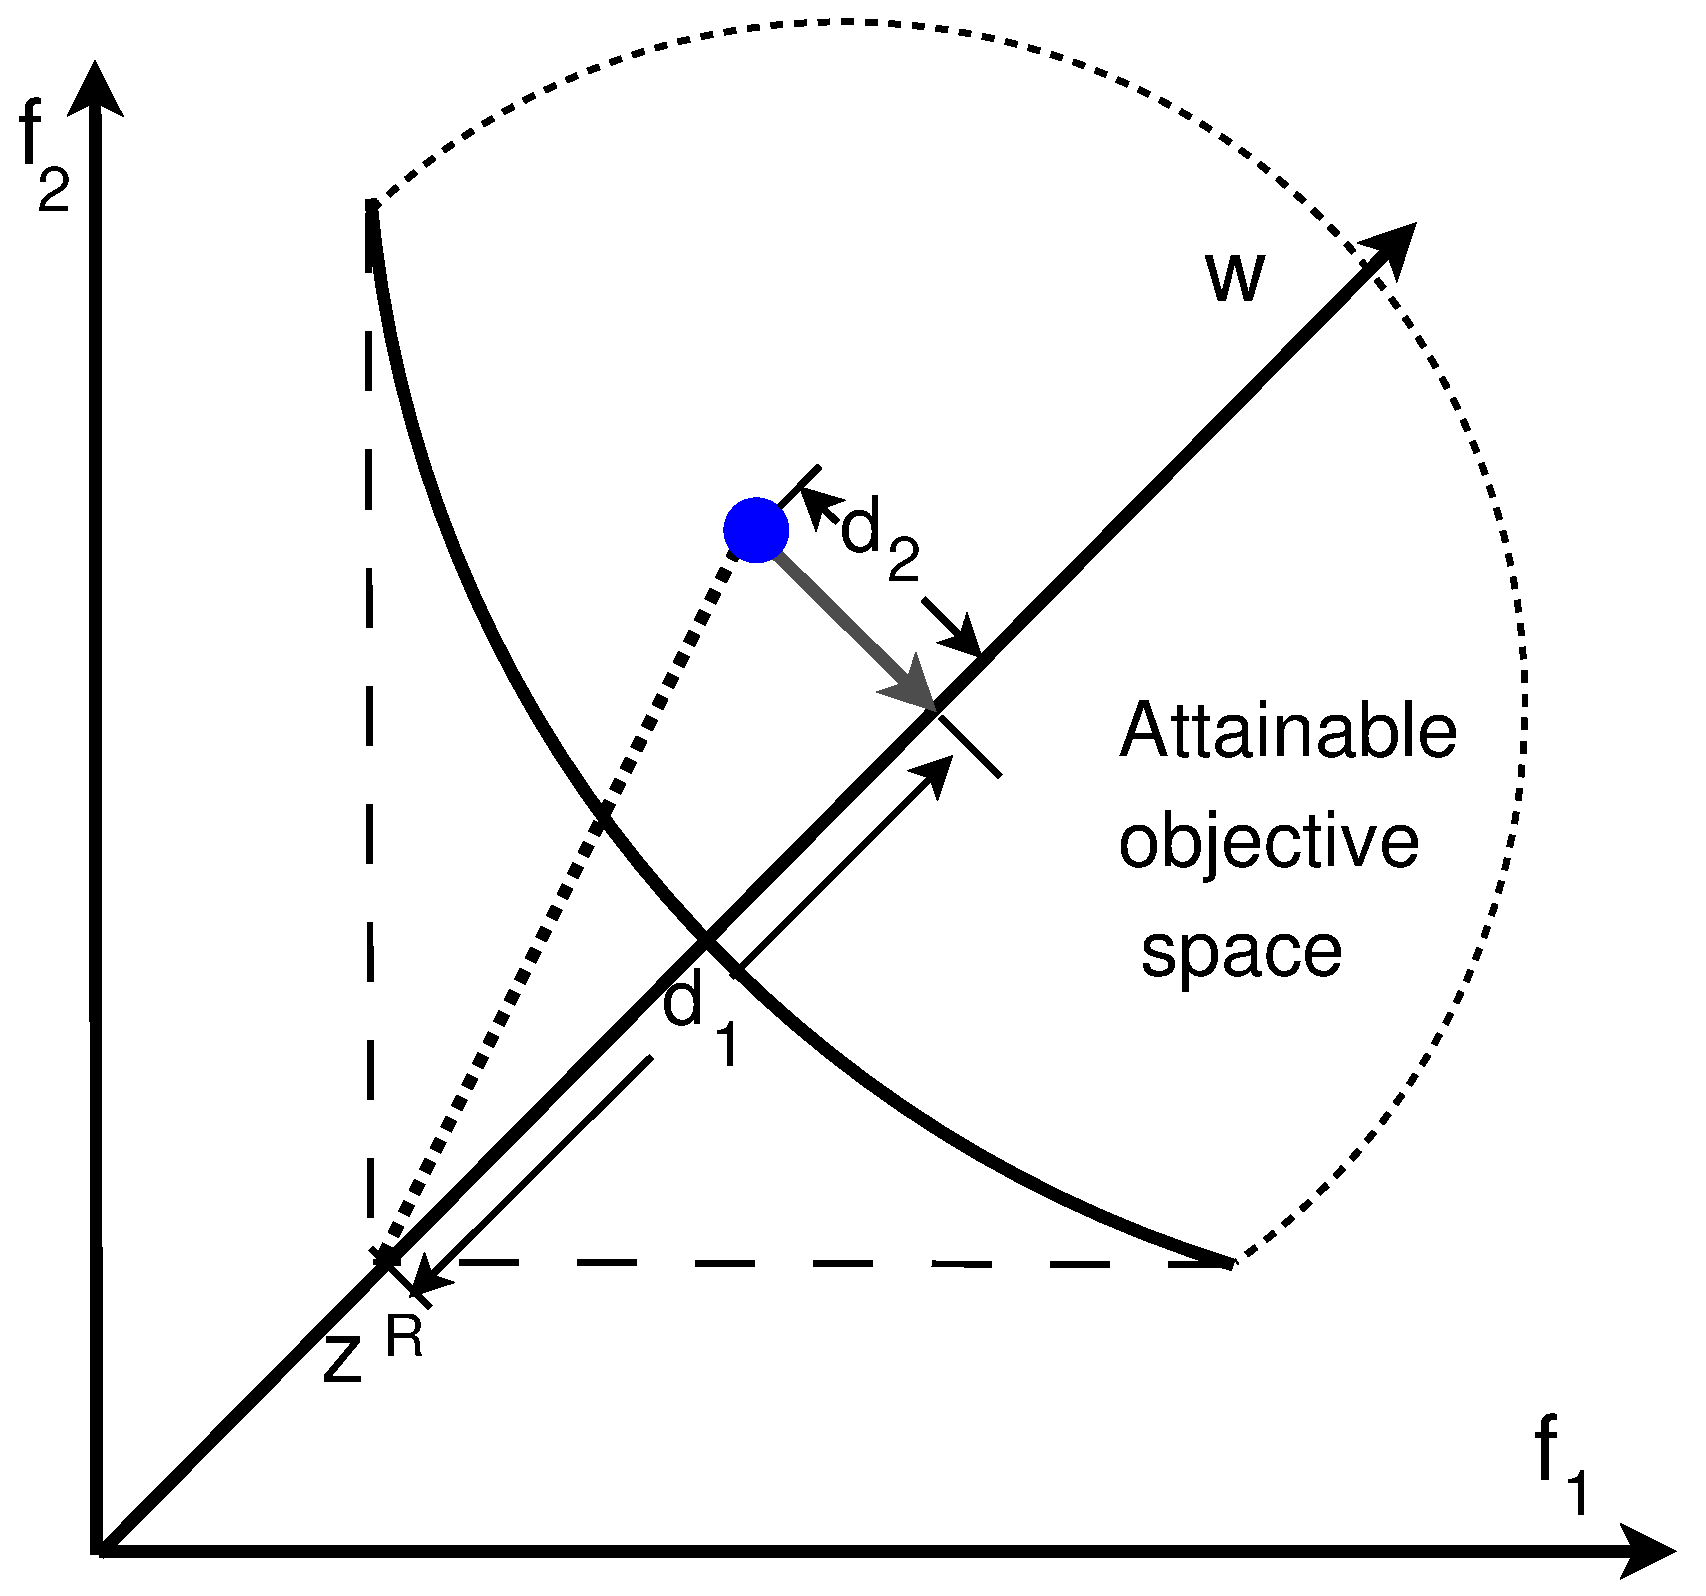
\includegraphics[width=1.3in]{figures/distance_example.eps}}\quad
\caption{(a) Uniform reference vectors; and (b) distance measures}
\label{fig:nbi}     
\end{center}
\end{figure}
\vspace{-1em}

%{\color{blue}There still remain a number of other current research issues regarding decomposition that need further development}. The first relates to the choice of reference directions themselves. The reference directions constructed by joining the ideal point to the systematically sampled points above favors certain shapes, colloquially referred to as ``regular'' PFs. \footnote{\color{blue} Regular PFs are typically those that are continuous, not highly non-linear and can be mapped easily using the uniform reference vectors on a triangular plane as shown in Fig.~\ref{fig:nbi_ref}. These include, for example, triangular PF and spherical PFs that have vertices on each of the objective axes. The PFs that do not conform to this type of geometry are referred to as irregular PFs, for example  disconnected, degenerated, highly convex/concave,``inverted'' triangle/sphere and other similar shapes}.  Secondly, presence of ``dominance resistant solutions~(DRS)'' is known to adversely affect scaling and design of robust and stable scaling schemes need further development. DRS refers to solutions which have extremely poor performance in one or more objectives, but remain non-dominated in the population due to extremely good performance in at least one other objective. The third issue relates to the need for reference vector adaptation, i.e., online re-distribution of reference vectors to deal with discontinuous, irregular and degenerate Pareto fronts. {\color{blue}These are some of the ongoing research directions in the field, though not the particular focus of this work}. For more detailed discussion on these issues, please refer to the recent papers \cite{asaf2017enhanced,KHTishibuchi2016inverse}.

\vspace{-0.3em}
\subsection{Surrogate assisted optimization}

Surrogate-assisted optimization, as the name reflects, attempts to use a ``surrogate'', i.e., an alternate approximation of the objective function/constraint under consideration. The technique has also been referred to using a number of other nomenclatures, such as meta-models, approximation models, empirical models, etc. If a good surrogate model can be built for a computationally expensive numerical function, then such a model can be used to guide the search in lieu of the true evaluations, resulting in potentially significant reduction in the optimization run-time. {\color{blue} One line of research in the area is the development of novel mathematical techniques to build accurate and generalizable surrogate models. Several approaches have been established in the literature towards this, such as radial basis functions, artificial neural networks, Kriging, which are reviewed in \cite{KHTjin2005csf,KHTjinswarm2011}, and a comparative analysis is presented in\cite{jin2001comparative}. Another key research direction~(and also the focus of this work) is on the ways of using surrogate models effectively to guide the search in classical or evolutionary algorithm. A comprehensive review of surrogate methods to support both type of engineering design optimization methods can be found in \cite{KHTwangreview2007}}. For the sake of brevity, we do not discuss them in detail here but instead summarize two of the key observations from existing literature. 
\vspace{-0.3em}
\begin{enumerate}

{\color{blue}
\item Majority of the works till date consider utilizing surrogate/metamodels to expedite the search for single-objective problems. There have also been increasing number of recent studies in dealing with multi-objective optimization problems~(up to 2/3 objectives)~\cite{Knowles2008}. However, as far as many-objective problems problems~($>4$ objectives) are concerned, the foray of surrogate-assisted methods is recent and so far there are only two published works~\cite{KHTchugh2016krvea,KHTchugh2016const} on it~(the former is applicable for unconstrained problems while the latter assumes constraints are cheap to evaluate and is never approximated). Single-objective algorithms work~(typically) relying on ranking based on a singular measure~(which can be predicted or evaluated), whereas multi-objective algorithms typically work based on Pareto-dominance~(of evaluated or predicted objective values). In our previous work~\cite{KHTjmd2016}, we had proposed and analyzed strategies for MOPs, comparing and contrasting them on various 2-3 objective problems. However, fundamentally, these~(and other methods with similar ranking strategies, such as \cite{KHTknowles2006pha}) do not scale up to MaOPs because Pareto-dominance based sorting is extensively used in the approach during selection~\cite{KHTishibuchi2008evolutionary}. In general, selection in MOP/MaOPs tends to be more complex than single-objective problems since both convergence and diversity of the solutions in the objective space needs to be considered.
}

%most of the existing literature deals primarily with single-objective optimization problems. While the approximation methods themselves can be applied to multiple objectives one at a time in the same way as that a single-objective problems, their integration in an evolutionary framework is not straightforward. The selection technique in presence of multiple objectives needs more careful consideration compared to the single-objective cases. The predicted values from the surrogate models need to be used in a way that promotes solutions that are likely to be good \emph{both} in convergence and diversity. Pareto-dominance technique has been primarily used for the selection in the existing surrogate assisted algorithms~(including authors' own)~\cite{KHTjmd2016,bhattacharjee2016multiple,KHTknowles2006pha}, which as discussed is not suitable for MaOPs. {\color{blue}To the authors' knowledge, the only dedicated attempt in this direction so far is the Kriging based Reference Vector Guided Evolutionary Algorithm~(K-RVEA) presented in \cite{KHTchugh2016krvea,KHTchugh2016const}~(the difference in the two being that the latter includes constraint handling).}  

\item It is also recognized widely now that no single surrogate is ubiquitously the best to approximate all types of functions. While the use of a single type of surrogate remains the general approach~(often based on preference/experience/familiarity with a particular type of surrogate),  the use of multiple surrogates has often proven to be advantageous. The common use of multiple surrogates is in the form of surrogate \textit{ensembles}~\cite{goel_ensemble_2007,zerpa_optimization_2005, hamza2012co}, where a collection of surrogate models with varying parameters are trained simultaneously by techniques such as bagging~\cite{breiman_bagging_1996} and boosting~\cite{abney_boosting_1999}. In the authors' previous works, multiple surrogates were employed for approximating the functions locally and the best one was chosen~\cite{KHTjmd2016,bhattacharjee2016multiple,KHTisaacs2009multi} in order to provide better flexibility of modeling the objectives/constraints of varying degrees of non-linearity. The general practice has been to use the same type of model for all functions involved in the problem, but recognizing that different functions might be better approximated by different {\color{blue}types} of models, some studies model them individually~\cite{KHTjmd2016,bhattacharjee2016multiple}. 

\end{enumerate}

\subsection{Motivation and scope}

The above discussions form the motivation of this study. The overall goal is to improve and analyze the state-of-the-art approaches for solving computationally expensive MaOPs. The paper presents a number of contributions towards this aim. 

\begin{itemize}

\item[$\bullet$] The first contribution is to extend the concept of multiple-surrogate assisted optimization for MaOPs. In our prior works, we have developed methods to tackle these challenges individually, but not together. For example, the paper on MaOP~\cite{KHTjmd2017} discussed a novel strategy for improving selection within a decomposition based evolutionary algorithm, but does not consider the objective/constraints to be computationally expensive. On the other hand, the work in \cite{KHTjmd2016,bhattacharjee2016multiple} uses multiple surrogates, {\color{blue}but it is not} suitable~(and not scalable) for MaOPs due to the use of Pareto-dominance. This work attempts to develop a decomposition based method with multiple surrogates to bridge this gap. 

\item[$\bullet$]  For effective selection of solutions to be evaluated~(considering very low evaluation budgets), apart from the ranking measures themselves, we embed a local search in the proposed approach. {\color{blue}The general idea is to use the approximated values effectively to identify solutions that are most likely to improve the quality of the current non-dominated set, \emph{before} performing true evaluations.} We compare and contrast two measures for these two operations, namely Achievement Scalarizing Function~(ASF) and Euclidean Distance~(ED), in order to provide more insights into the working of the algorithm. 


\end{itemize}

{\color{blue}
In order to demonstrate the effectiveness of the proposed approach, comparisons are performed with the recently proposed K-RVEA algorithm~\cite{KHTchugh2016krvea,KHTchugh2016const} and the well known ParEGO algorithm~\cite{KHTknowles2006pha}. In-line with the recent observations~\cite{asaf2017enhanced,KHTishibuchi2016inverse} that ``regular'' problems are not sufficient to reliably evaluate the algorithms' performance, we use a large problem set containing both regular and inverted PFs for a more extensive comparison. Lastly, we present a case study involving {\color{blue}vehicle design} as a simulated real-life optimization problem to illustrate the benefits of such an approach. 
}


\section{Surrogate assisted multi-objective Optimization}
\label{sec:KHTsec:3}

The proposed algorithm is based on a ($\mu$ + $\lambda$) evolutionary model, where $\mu$ parents are recombined to generate $\lambda$ offspring and the best $\mu$ solutions are selected as the next generation population. The general framework of the proposed method, referred to as \textit{Surrogate Assisted Many-objective Optimization~(SaMaO)} is presented in Algorithm~\ref{alg:KHTAlgo:1}. The details of its key components are outlined in the following subsections. 


\begin{algorithm}[!ht]\footnotesize
	\caption{SaMaO}
	\textbf{Input:} $TFE_{max}$\hspace{1mm}(Total true function evaluations budget), $N_I$\hspace{1mm}(Initial population size), $N$\hspace{1mm}(Population size during evolution i.e. $\mu$), $K$\hspace{1mm}(Max. number of true evaluations in each generation)
	\begin{algorithmic}[1]
		\STATE $TFE$ = 0, $j$ = 1, Archive of truly evaluated solutions $\mathcal{A}$ = $\emptyset$
		\STATE \textbf{Generate} initial reference vector set $W$ 
		\STATE $P^I$ = \textbf{Initialize}(), $\left|P^I\right| = N_I$ 
		\STATE \textbf{Evaluate} every objective and constraints of $P^I$, Update $TFE$, $\mathcal{A}$ 
%		\STATE \textbf{Add} $P^j$ to archive~($\mathcal{A}$)
		\STATE \textbf{Build} global surrogate models for each objective and constraint
		\STATE $W_m$ = \textbf{UpdateRef}($W$,$\mathcal{A}$)
		\STATE $P^j$ = \textbf{Assign}($W_m$,$P^I$) 	
		\WHILE{$(TFE\le TFE_{max})$}
		\STATE $C$ = \textbf{CreateOffspring}($P^j$), $\left|C\right|$ = $N$
		\STATE \textbf{Approximate} each objective function and each constraint function of $C$
		\STATE $C_K$ = \textbf{Identify}($P^j$,$C$,$\mathcal{A}$), $\left|C_K\right| \le K$
		\STATE \textbf{Evaluate} every objective and constraint of $C_K$, Update $TFE$, $\mathcal{A}$
%		\STATE \textbf{Add} $C_K$ to archive~($\mathcal{A}$)
		\STATE \textbf{Build} global surrogate models for each objective and constraint
		\STATE \textbf{Approximate} each objective function and each constraint function of $C \setminus C_K$
		\STATE $W_m$ = \textbf{UpdateRef}($W$,$P^j \cup C \setminus C_K \cup C_K$)
		\STATE $P^{j+1}$ = \textbf{Assign}($W_m$,$P^j \cup C \setminus C_K \cup C_K$)   
		\STATE $j$ = $j$ + 1
		\ENDWHILE			
		
	\end{algorithmic}
	\label{alg:KHTAlgo:1}
\end{algorithm}

The key steps of the algorithm~(highlighted in bold) are elaborated below:\\

\noindent \underline{\it \textbf{Generate}}: A structured set of $W$ reference points is generated using the method of systematic sampling~(normal boundary intersection~(NBI)) as commonly adopted in decomposition based approaches in the literature~\cite{KHTdas1998normal,KHTjmd2017,KHTtrivedisurvey}. The approach generates $W$ points on the hyperplane in $M$-objective space with a uniform spacing of $\delta=1/H$ with $H$ unique sampling locations along each objective axis. The reference directions are formed by joining the ideal point~(origin in the scaled space) to each of these reference points. In this approach, $N = {H+M-1}\choose{M-1}$ reference directions are generated. However, for larger number of objectives, a two-layered approach is commonly used in the field~(and adopted here) which is defined using $H_1$ and $H_2$ as outlined in \cite{KHTLi2015dominance}. Such an approach limits the number of reference points from growing exponentially with respect to $M$.

	\noindent \underline{\it \textbf{Initialize}}: $N_I$ solutions are initialized within the variable bounds $\textbf{x}^{L}$ and $\textbf{x}^{U}$ using the space-filling Latin Hypercube Sampling based on ``maximin'' criterion.
	
	\noindent \underline{\it \textbf{Evaluate}}: In this stage, the objective functions and constraint functions~(if present) are truly evaluated for all the solutions generated above. {\color{blue}Subsequently~(and whenever a new solution is evaluated)}, the archive of truly evaluated solutions $\mathcal{A}$ is updated. 
	
	
	\noindent \underline{\it \textbf{Build}}: This process involves building the surrogate models for each objective and constraint function using different types of approximation methods: Radial Basis Function~(RBF), Kriging and Response Surface Methodology~(RSM) of $1^{st}$ and $2^{nd}$ order. From these, 80\% of the solutions are selected based on ``k-medoid'' clustering to train the surrogate models, while the rest are used for validation. Take note that for model building, the variables are scaled between 0 and 1 using the bounds $\textbf{x}^{L}$ and $\textbf{x}^{U}$ and the same applies for clustering. Mean squared error~(MSE) based on the validation set~(i.e., the remaining 20\% solutions) is used to choose the most appropriate surrogate model for each objective function. 
	
	\noindent \underline{\it \textbf{UpdateRef}}: In this stage, the $i^{th}$ reference direction $W^i$ is modified to $W^i_m$ based on the ideal vector ($Z^I$) and nadir vector ($Z^N$) of the combined parent, child and archive population using Equation \ref{eqn:KHTEqn:3}. Take note that  the proposed approach uses the nadir point of the combined parent, child and archive population as opposed to the use of parent and child population only in the Reference Vector guided Evolutionary Algorithm~\cite{KHTCheng2016many}. This approach has the benefits of relying on mixed bag of solutions (both actually evaluated and predicted) instead of relying only on predicted set of solutions. The advantage of using both together for selection has been demonstrated in our earlier work~\cite{bhattacharjee2016multiple} for MOPs.
	
	\begin{equation}\footnotesize
	(W^i_m)_j = (W^i)_j\times(Z^N - Z^I)_j, \forall~1\le j\le M
	\label{eqn:KHTEqn:3}
	\end{equation}
	
\noindent \underline{\it \textbf{Assign}}: In this stage, solutions are assigned to the reference directions. Let the number of solutions to be assigned be denoted by $R$, of which $R1$ and $R2$ are the numbers of feasible and infeasible solutions respectively. If $R < N$, then additional random copies of $R1$ solutions are created. This would result in a current population with $N-R2$ feasible solutions and $R2$ infeasible solutions. If the number of solutions to be assigned is more than $N$, the solutions are first grouped into feasible and infeasible solutions. If the number of feasible solutions exceeds the population size~($N$), the feasible solutions are assigned using the assignment strategy of RVEA, albeit with different metrics (ASF and normalized Euclidean distance from the ideal point (ED)) for different algorithm instances~(discussed shortly). Otherwise, ``feasibility first'' principle is applied to select top $N$ solutions. Take note that, in the assignment process of the feasible solutions, a sub-population with respect to a reference direction is constructed using the solutions which are closest to that reference direction. The closeness is based on angle formed between the reference vector and the direction formed by joining the solution with the ideal point. If no solutions belong to a sub-population, it is considered empty. 
	
\noindent \underline{\it \textbf{CreateOffspring}}: The process of creating offspring solutions involves two steps, the identification of participating parents for recombination and the recombination process itself. Both these steps are known to affect the performance and various rationales and recommendations have been suggested in the literature. In our approach, if all solutions in the population are feasible, each solution is selected as a base parent and its partner is randomly chosen from the rest. Such a scheme offers opportunity to all solutions to act as base parents for generating offspring.
	
Next, let us consider the second case where a population contains a mix of feasible and infeasible solutions. Most algorithms adopt a feasible first strategy, i.e., feasible solutions are ranked explicitly above the infeasible solutions~\cite{deb2001multi}. However, ranking all feasible solutions above all infeasible solutions in the ordered list has important implications\cite{KHTSingh2013idea}. Ideally, a marginally infeasible solution might be closer to the true optimum, which often lies on a constraint boundary, and allowing participation of such solutions would be more beneficial than using a feasible solution away from the true optimum, as investigated in a number of recent studies~\cite{KHTsingh2016use}. An ordering scheme which places marginally infeasible solutions at the top of the ranked list of solutions appears in \cite{KHTSingh2013idea,KHTRay2009idea}. The same scheme has been used in the proposed approach to order the solutions which subsequently engage in a binary tournament resulting in a set of $\mu$ base parents. It is important to highlight that preservation of marginally infeasible solutions is known to significantly improve the rate of convergence of optimization algorithms as reported in the literature~\cite{KHTsingh2016use, KHTtakahama2005constrained,KHTRay2009idea}. One participating parent for each base parent is selected randomly from the list of $\mu$ base parents. Once the base parent and participating parent is identified, two offspring are generated using simulated binary crossover and polynomial mutation of which a random offspring is selected.  
	
\noindent \underline{\it \textbf{Approximate~(predict)}}: {\color{blue}This stage involves predicting the approximate value of each objective and constraint function using the best surrogate i.e one with the minimum MSE on the validation set.}
	
\noindent \underline{\it \textbf{Identify}}: Given that the computational budget is very limited, the selection of solutions to be truly evaluated needs significant consideration, such that significant improvements in convergence and diversity of the solutions could be achieved. This step of the algorithm is aimed at identifying at most $K$ solutions for actual evaluation from the combined pool of parent and offspring solutions. Based on the feasibility status of the solutions, three situations may arise: (a) If there are no feasible solutions in the combined pool, $K$ is set to be zero, i.e, no new solutions are evaluated;  (b) If the number of feasible solutions in the combined pool is less than $K$, the feasible solutions are evaluated using actual evaluations if they are not available from the archive; (c) If there exist more than $K$ feasible solutions in the combined pool which are not members of the archive, the following steps are used to identify the required $K$ solutions. The feasible solutions belonging to the combined pool and the archive are used to construct sub-populations using updated reference directions. Thereafter, solutions with the best value of a given fitness metric~(such as ASF, ED) are selected from the members of each non-empty sub-population. However, in the context of an empty sub-population, solution with the best value of the metric is selected from all the feasible solutions belonging to the combined pool and the archive. This results in $N$ assigned solutions. If all $N$ solutions in this stage are members of the archive ($\mathcal{A}$), the following steps are performed with only offspring solutions as opposed to the combined pool of solutions. A local search is performed from each of these assigned solutions as the starting point to identify a better solution where the objective is to obtain the best value of fitness metric subjected to an angle constraint. The angle constraint ensures that the angle between any feasible solution and the reference direction associated with the best solution is always less than the minimum angle between that reference direction and {\color{blue}its neighboring} reference directions; to ensure diversity. The reference directions corresponding to the non-empty sub-populations are clustered into $K$ regions based on ``k-medoid'' clustering. For each cluster, the reference directions as well as their associated solutions are identified. Then, the best solution in each cluster is identified as the solution having minimum fitness metric. The associated reference direction with the best solution is also identified. Finally, a local search is performed from each of these best solutions as the starting point to identify a better solution where the objective is to minimize the ED or ASF value subjected to an angle constraint. Out of these $K$ solutions obtained after local search, the ones that are not members of the archive ($\mathcal{A}$) are identified and evaluated.    

As noted above, a performance metric is needed for selection in the above process, as well as during the local search. In this study we consider two performance metrics: Achievement Scalarizing Function~(ASF), and the Euclidean Distance~(ED). We study three combinations - one where ASF is used for both~(denoted as SaMaO\textsubscript{ASF-ASF}), another where ED is used for both~(SaMaO\textsubscript{ED-ED}), and third one where ASF is used for selection and ED for local search~(SaMaO\textsubscript{ASF-ED}). We show empirically later on that using the third strategy~(SaMaO\textsubscript{ASF-ED}) yields the best results and explain why it is so.

The above process runs in a loop until the prescribed budget on the true function evaluations~($TFE_{max}$) is exhausted, and the resulting non-dominated set from all truly evaluated solutions by the algorithm is presented as the final output from the optimization run. In the next section, we test the strategy on several benchmark problems to demonstrate its competence comprehensively. 

\section{Numerical Experiments}
\label{sec:KHTsec:4}

The numerical experiments are detailed in this section. We start with a brief outline of the problems considered and the performance metrics, followed by the experimental setup and results. 

\subsection{Problems and Performance metric}

The most commonly studied benchmarks in the field of MaOPs have been the DTLZ series~(named after the authors Deb, Thiele, Laumanns, Zitzler)~\cite{KHTdeb2005scalable}, and WFG~(Walking Fish Group)~\cite{KHTwfg2006huband} series problems, both of which are scalable in terms of decision variables as well as objectives. In general, the latter series is deemed to be somewhat more difficult to solve than the former, but both the series share one common property that makes them conducive use of traditional decomposition based methods. Most of the problems in these series have linear/quadratic PFs which are oriented such that they can be mapped well by the traditional way of generating reference vectors on a hyperplane~(as shown in Fig.~\ref{fig:nbi}). It has been revealed and discussed in-depth in some of the recent papers\cite{asaf2017enhanced,KHTishibuchi2016inverse} that the performance of the decomposition based approaches strongly depends on the shape of the PF, and hence testing them on the regular problems alone may form an incomplete picture of an algorithm's performance. A series of problems with so called ``inverted'' PFs was therefore proposed in  \cite{KHTishibuchi2016inverse}, which are referred to as the ``minus'' problems. For a comprehensive evaluation of the presented approach, we therefore use a comprehensive set of test problems from both the original~(DTLZ1-DTLZ7, WFG1-WFG9) and the minus sets~(DTLZ1\textsuperscript{-1}-DTLZ4\textsuperscript{-1},WFG1\textsuperscript{-1}-WFG9\textsuperscript{-1}) with up to 10-objectives. The number of decision variables are kept the same as those recommended in \cite{KHTchugh2016krvea} for DTLZ and WFG problems. For the minus problems, the number of decision variables suggested in \cite{KHTishibuchi2016inverse} are used.  In addition, we also present a practical application of a 5-objective {\color{blue}vehicle design} problem~\cite{KHTbarnum2010car}. The number of decision variables for the {\color{blue}vehicle design} problem is 10.

Since the optimum of MOPs/MaOPs comprise not one but a set of designs, for a quantitative comparison, metrics that capture convergence and diversity of the PF approximation are required. One such widely used metric, Inverted Generational Distance~(IGD), is considered in this paper for performance comparisons. IGD calculates the average distance of the closest points obtained with respect to a reference set which is a close representation of the true PF. Since the true PF is known for the benchmark problems, a sufficiently large set of points can be sampled on the PF to construct the reference set. In this study, we use the same IGD reference those in \cite{KHTchugh2016krvea,KHTchugh2016const} for DTLZ, WFG and CDTLZ series problems. For the minus problems~(those with inverted PF), we have constructed the reference sets from their original counterparts, DTLZ and WFGs and inverted them. The size of the IGD reference sets are listed in Table~\ref{tab:KHTTab:1}. 

{\color{blue} In addition to IGD, we have also for the first time included performance of the approaches based on hypervolume~(HV) measures. As for hypervolume, the choice of the reference point used for HV computation is crucial and can adversely affect the interpretations about relative performance~\cite{KHTYuan2016many,KHTishibuchi2010many}. For HV computation, there are recent reports that suggest use of a slightly larger than true nadir vector as a reference point~\cite{KHTYuan2016many,KHTishibuchi2010many}. In our experiments, we have used the reference point to be 1.1 multiplied by the theoretical nadir vector for problems. Given a set of solutions and their corresponding objective vectors, we first discard all solutions that are dominated by the reference point. The objective vectors of the remaining solutions are normalized using the ideal and the modified nadir vector and HV is computed using a reference point which is $1.1^M$ in the normalized space~($M$ is the number of objectives). All HV computations reported in this paper are based on exact method~(WFG algorithm)~\cite{KHTwhile2012hv}. HV and IGD computations in this paper are based on solutions obtained from the archive i.e. the set of all fully evaluated solutions so far. }

\begin{table}[!htb]\scriptsize
	\centering
	\caption{Number of points in the reference set for IGD calculation}
	\label{tab:KHTTab:1}
	\tabcolsep = 0.03cm
	\begin{tabular}{|c|c|c|c|}
		\noalign{\smallskip}\hline
\textbf{M} &\parbox[t]{5cm}{\centering\textbf{DTLZ1-DTLZ6, WFG1, WFG3-WFG9, DTLZ1\textsuperscript{-1}-DTLZ4\textsuperscript{-1}, WFG1\textsuperscript{-1}, WFG3\textsuperscript{-1}-WFG9\textsuperscript{-1}}} & \textbf{DTLZ7} & \parbox[t]{1cm}{\centering\textbf{WFG2,\\ WFG2\textsuperscript{-1}}}\\ \hline
 3          & 5050                                                                                                                                                                              & 6084           & 4101                                      \\ \cline{1-4} 
	 4          & 10660                                                                                                                                                                             & 10648          & 10708                                     \\ \cline{1-4} 
	 6          & 33649                                                                                                                                                                             & 59049          & 32191                                     \\ \cline{1-4} 
	 8          & 50388                                                                                                                                                                             & 78125          & 66342                                     \\ \cline{1-4} 
	 10         & 92378                                                                                                                                                                             & 262144         & 115610                                    \\ \hline

\end{tabular}
\end{table}

\subsection{Experimental setup and results}
\label{subsec:KHTsubsec:2}
In all the examples presented in this study, the probability of crossover is set to 0.9 and the probability of mutation is set to $\frac{1}{n}$ ($n$ is the number of variables for each problem). The distribution index for crossover is set to 30 and the distribution index for mutation is set to 20. To build the surrogates, 80\% of the solutions are used for training and rest for validation. Take note that the surrogates are constructed on the scaled variable space. The types of approximations include 1$^{st}$ and 2$^{nd}$ order response surface method, Kriging and radial basis function networks. The size of the initial population is set as $(11\times n)-1$ for all the problems. Sequential quadratic programming (SQP) in MATLAB 2015b is used as the solver for the local search. The maximum number of iterations and the maximum number of function evaluations in the context of SQP are considered to be 1000 and 1000 respectively. All the other parameters for SQP are considered to be the same as the default in MATLAB 2015b. The maximum allowable cost~($TFE_{max}$) is set to 300 for all benchmark problems. Five solutions are at most evaluated in every generation, i.e., $K = 5$ for all benchmark problems. The results reported for each benchmark problem are based on 25 independent optimization runs. Best results in terms of mean IGD values are marked in bold for all the instances of all the benchmark problems. $K = 10$ is considered for the engineering design problem and $TFE_{max}$ is set to 4000.

The results obtained using different variants of SaMaO are compared amongst themselves for DTLZ and WFG problem instances and minus problems~(3, 4, 6, 8 and 10-objective). The best variant based on significance test is compared with the existing algorithms, namely K-RVEA~\cite{KHTchugh2016krvea}, RVEA~\cite{KHTCheng2016many} and ParEGO~\cite{KHTknowles2006pha} for unconstrained DTLZ and WFG problem instances~(3, 4, 6, 8 and 10-objective) and with K-RVEA for minus problems. Results of K-RVEA were generated using the codes from \cite{KHTplatemo}. The results for RVEA and ParEGO were obtained from \cite{KHTchugh2016krvea}. A Wilcoxon rank sum test was also used to compare the results obtained by the variants of proposed approach (SaMaO) and K-RVEA on all unconstrained problems at a significance level of 0.05. 

\subsubsection{Benchmark problems}
The detailed results are included in the online supplementary material. Here, we present the summary based on the results of significance test based on IGD and HV for DTLZ and WFG and thereafter their minus counterparts. 


\begin{table*}[!htb]\scriptsize
	\centering
	\caption{Significance Tests based on IGD for conventional DTLZ \& WFG problems. Total number of problems = 16; total instances = 16$\times$5=80}
	\label{tab:KHTTab:4}
	\tabcolsep = 0.03cm
	\begin{tabular}{|c|c|c|c|c|c|c|c|c|c|c|c|c|c|c|c|}
		\hline
		\textbf{M}&\multicolumn{3}{|c|} {SaMaO\textsubscript{ASF-ED} vs SaMaO\textsubscript{ASF-ASF}} & \multicolumn{3}{|c|} {SaMaO\textsubscript{ASF-ASF} vs SaMaO\textsubscript{ED-ED}} & \multicolumn{3}{|c|} {SaMaO\textsubscript{ED-ED} vs SaMaO\textsubscript{ASF-ED}}&  \multicolumn{3}{|c|} {SaMaO\textsubscript{ASF-ED} vs K-RVEA}\\
		\hline
		                   & \textbf{SaMaO\textsubscript{ASF-ED}} & \textbf{SaMaO\textsubscript{ASF-ASF}} & \textbf{Equivalent}  & \textbf{SaMaO\textsubscript{ASF-ASF}} & \textbf{SaMaO\textsubscript{ED-ED}} & \textbf{Equivalent} & \textbf{SaMaO\textsubscript{ED-ED}} & \textbf{SaMaO\textsubscript{ASF-ED}} & \textbf{Equivalent}& \textbf{SaMaO\textsubscript{ASF-ED}} & \textbf{K-RVEA} & \textbf{Equivalent}\\ \hline
		\textbf{3}                   & 0                             & 2                              & 14             & 4                              & 1                            & 11               & 2                            & 2                             & 12          & 10                            & 1                       & 5                   \\ \hline
		\textbf{4}                   & 2                             & 7                              & 7                    & 9                              & 2                            & 5        & 2                            & 6                             & 8    	 & 12                            & 2                       & 2                   \\ \hline
		\textbf{6}                   & 5                             & 4                              & 7                  & 7                              & 3                            & 6     & 0                            & 5                             & 11                        & 7                             & 5                       & 4                   \\ \hline
		\textbf{8}                   & 7                             & 2                              & 7                   & 6                              & 6                            & 4       & 1                            & 8                             & 7            & 10                            & 2                       & 4                   \\ \hline
		\textbf{10}                  & 10                            & 3                              & 3                  & 4                              & 9                            & 3 	     & 4                            & 4                             & 8                          & 7                             & 3                       & 6                   \\ \hline   
	\end{tabular}
\end{table*}


\begin{table*}[!htb]\scriptsize
	\centering
	\caption{Significance Tests based on HV for DTLZ \& WFG problems. Total number of problems = 16; total instances = 16$\times$5=80}
	\label{tab:KHTTab:10}
	\tabcolsep = 0.03cm
	\begin{tabular}{|c|c|c|c|c|c|c|c|c|c|c|c|c|c|c|c|}
		\hline
		\textbf{M}&\multicolumn{3}{|c|} {SaMaO\textsubscript{ASF-ED} vs SaMaO\textsubscript{ASF-ASF}} & \multicolumn{3}{|c|} {SaMaO\textsubscript{ASF-ASF} vs SaMaO\textsubscript{ED-ED}} & \multicolumn{3}{|c|} {SaMaO\textsubscript{ED-ED} vs SaMaO\textsubscript{ASF-ED}}&  \multicolumn{3}{|c|} {SaMaO\textsubscript{ASF-ED} vs K-RVEA}\\
		\hline
		& \textbf{SaMaO\textsubscript{ASF-ED}} & \textbf{SaMaO\textsubscript{ASF-ASF}} & \textbf{Equivalent}  & \textbf{SaMaO\textsubscript{ASF-ASF}} & \textbf{SaMaO\textsubscript{ED-ED}} & \textbf{Equivalent} & \textbf{SaMaO\textsubscript{ED-ED}} & \textbf{SaMaO\textsubscript{ASF-ED}} & \textbf{Equivalent}& \textbf{SaMaO\textsubscript{ASF-ED}} & \textbf{K-RVEA} & \textbf{Equivalent}\\ \hline		
		\textbf{3}                   & 1                             & 1                              & 14          & 3                      & 0                    & 13              & 0                    & 3                     & 13         & 8                             & 3                              & 5           \\ \hline
		\textbf{4}                   & 3                             & 4                              & 9            & 6                      & 2                    & 8                   & 0                    & 5                     & 11        & 6                             & 3                              & 7         \\ \hline
		\textbf{6}                   & 3                             & 4                              & 9            & 6                      & 3                    & 7                & 1                    & 3                     & 12              & 4                             & 6                              & 6              \\ \hline
		\textbf{8}                   & 3                             & 2                              & 11              & 7                      & 3                    & 6               & 1                    & 6                     & 9                    & 5                             & 2                              & 9      \\ \hline
		\textbf{10}                  & 6                             & 1                              & 9             & 6                      & 4                    & 6                & 2                    & 7                     & 7            & 5                             & 5                              & 6          \\ \hline
	\end{tabular}
\end{table*}

Table~\ref{tab:KHTTab:4} shows pair-wise comparisons between the three variants of SaMaO in terms of statistical tests(Wilcoxon rank-sum) based on IGD. It can be seen that SaMaO\textsubscript{ASF-ED} is significantly better than the other two variants for a total of 49 instances; whereas SaMaO\textsubscript{ASF-ASF} and SaMaO\textsubscript{ED-ED} are better for 48 and 30 instances respectively. It is clear based on the significance tests on IGD that the best variant is SaMaO\textsubscript{ASF-ED} which is then further compared with K-RVEA in terms of significance tests. The significance test from Table \ref{tab:KHTTab:4} reveals that the proposed approach delivers significantly better results in 46 out of 80 instances and equivalent results in 21 out of 80 instances compared to K-RVEA. Note that since the performance delivered using RVEA and ParEGO are obtained from~\cite{KHTchugh2016krvea} which consists of only best, mean and worst IGD values, the significance test could not be performed with these approaches. One can also observe from Table~\ref{tab:KHTTab:4}, SaMaO\textsubscript{ASF-ED} performs the best. \textcolor{red}{Similarly Table~\ref{tab:KHTTab:10} shows the Wilcoxon rank-sum test among SaMaO variants, and K-RVEA with SaMaO\textsubscript{ASF-ED} based on HV for DTLZ and WFG series problems. One can observe that the proposed approach delivers significantly better results in 28 out of 80 instances and equivalent results in 33 out of 80 instances compared to K-RVEA, while it is worse than K-RVEA in merely 19 instances.}


Next we present the results for the minus problems. Similar to above, the comparison is carried out between the three variants of SaMaO and K-RVEA for 3, 4, 6, 8 and 10 objective instances of DTLZ1\textsuperscript{-1}-DTLZ4\textsuperscript{-1} and WFG1\textsuperscript{-1}-WFG9\textsuperscript{-1} problems. The significant test results amongst different variants of SaMaO based on IGD are provided in Table \ref{tab:KHTTab:12}. It is clear that SaMaO\textsubscript{ASF-ED} is again the best performing variant among the three. Therefore, this variant is then further compared with K-RVEA are presented in Table \ref{tab:KHTTab:12}. The comparisons reveals that the SaMaO\textsubscript{ASF-ED} delivers significantly better results in 26 out of 65 instances and equivalent results in 29 out of 65 instances compared to K-RVEA, while it is worse than K-RVEA in merely 10 instances. \textcolor{red}{Similarly Table~\ref{tab:KHTTab:11} shows the Wilcoxon rank-sum test among SaMaO variants, and K-RVEA with SaMaO\textsubscript{ASF-ED} based on HV on the minus problems. One can observe that the proposed approach delivers significantly better results in 32 out of 65 instances and equivalent results in 24 out of 80 instances compared to K-RVEA, while it is worse than K-RVEA in merely 9 instances.}

\begin{table*}[!htb]\scriptsize
	\centering
	\caption{Significance Test based on IGD for inverted (DTLZ\textsuperscript{-1} \& WFG\textsuperscript{-1}) problems. Total number of problems = 13; total instances = 13$\times$5=65}
	\label{tab:KHTTab:12}
	\tabcolsep = 0.03cm
	\begin{tabular}{|c|c|c|c|c|c|c|c|c|c|c|c|c|c|c|c|}
		\hline
		\textbf{M}&\multicolumn{3}{|c|} {SaMaO\textsubscript{ASF-ED} vs SaMaO\textsubscript{ASF-ASF}} & \multicolumn{3}{|c|} {SaMaO\textsubscript{ASF-ASF} vs SaMaO\textsubscript{ED-ED}} & \multicolumn{3}{|c|} {SaMaO\textsubscript{ED-ED} vs SaMaO\textsubscript{ASF-ED}}&  \multicolumn{3}{|c|} {SaMaO\textsubscript{ASF-ED} vs K-RVEA}\\
		\hline
		                   & \textbf{SaMaO\textsubscript{ASF-ED}} & \textbf{SaMaO\textsubscript{ASF-ASF}} & \textbf{Equivalent}  & \textbf{SaMaO\textsubscript{ASF-ASF}} & \textbf{SaMaO\textsubscript{ED-ED}} & \textbf{Equivalent} & \textbf{SaMaO\textsubscript{ED-ED}} & \textbf{SaMaO\textsubscript{ASF-ED}} & \textbf{Equivalent}& \textbf{SaMaO\textsubscript{ASF-ED}} & \textbf{K-RVEA} & \textbf{Equivalent}\\ \hline		
		\textbf{3}                   & 0                             & 1                              & 12          & 3                      & 1                    & 9              & 2                    & 2                     & 9         & 6                             & 1                              & 6           \\ \hline
		\textbf{4}                   & 1                             & 1                              & 11            & 3                      & 1                    & 9                   & 1                    & 3                     & 9        & 5                             & 2                              & 6          \\ \hline
		\textbf{6}                   & 0                             & 1                              & 12            & 4                      & 1                    & 8                & 1                    & 1                     & 11              & 2                             & 4                              & 7              \\ \hline
		\textbf{8}                   & 0                             & 0                              & 13              & 8                      & 0                    & 5               & 1                    & 5                     & 7                    & 6                             & 2                              & 5      \\ \hline
		\textbf{10}                  & 0                             & 1                              & 12             & 8                      & 0                    & 5                & 0                    & 5                     & 8            & 7                             & 1                              & 5          \\ \hline
	\end{tabular}
\end{table*}


\begin{table*}[!htb]\scriptsize
	\centering
	\caption{Significance Test based on HV for DTLZ\textsuperscript{-1} \& WFG\textsuperscript{-1} problems. Total number of problems = 13; total instances = 13$\times$5=65}
	\label{tab:KHTTab:11}
	\tabcolsep = 0.03cm
	\begin{tabular}{|c|c|c|c|c|c|c|c|c|c|c|c|c|c|c|c|}
		\hline
		\textbf{M}&\multicolumn{3}{|c|} {SaMaO\textsubscript{ASF-ED} vs SaMaO\textsubscript{ASF-ASF}} & \multicolumn{3}{|c|} {SaMaO\textsubscript{ASF-ASF} vs SaMaO\textsubscript{ED-ED}} & \multicolumn{3}{|c|} {SaMaO\textsubscript{ED-ED} vs SaMaO\textsubscript{ASF-ED}}&  \multicolumn{3}{|c|} {SaMaO\textsubscript{ASF-ED} vs K-RVEA}\\
		\hline
		& \textbf{SaMaO\textsubscript{ASF-ED}} & \textbf{SaMaO\textsubscript{ASF-ASF}} & \textbf{Equivalent}  & \textbf{SaMaO\textsubscript{ASF-ASF}} & \textbf{SaMaO\textsubscript{ED-ED}} & \textbf{Equivalent} & \textbf{SaMaO\textsubscript{ED-ED}} & \textbf{SaMaO\textsubscript{ASF-ED}} & \textbf{Equivalent}& \textbf{SaMaO\textsubscript{ASF-ED}} & \textbf{K-RVEA} & \textbf{Equivalent}\\ \hline		
		\textbf{3}                   & 0                             & 3                              & 10          & 1                      & 1                    & 11              & 3                    & 1                     & 9         & 8                             & 3                              &  2          \\ \hline
		\textbf{4}                   & 2                             & 1                              & 10            & 4                      & 1                    & 8                   & 0                    & 5                     & 8        & 4                             & 3                              & 6        \\ \hline
		\textbf{6}                   & 1                             & 0                              & 12            & 6                      & 0                    & 7                & 0                    & 6                     & 7              & 4                             & 1                              & 8              \\ \hline
		\textbf{8}                   & 0                             & 0                             & 13              & 7                      & 1                    & 5               & 0                    & 7                     & 6                    & 8                             & 1                              & 4      \\ \hline
		\textbf{10}                  & 1                             & 2                              & 10             & 8                      & 1                    & 4                & 2                    & 8                    & 3            & 8                             & 1                              & 4          \\ \hline
	\end{tabular}
\end{table*}


Thus, from the numerical experiments on a range of benchmark problems with both regular and inverted PFs, SaMaO\textsubscript{ASF-ED} convincingly outperforms the other two strategies~(SaMaO\textsubscript{ASF-ASF} and SaMaO\textsubscript{ED-ED}), as well as the other existing algorithms including the most recently proposed K-RVEA. 

The improved performance of SaMaO\textsubscript{ASF-ED} can be explained by observing the behavior of these two metrics closely. For any given point $\mathbf{f}$, reference vector $\mathbf{w}$ and a reference point $\mathbf{z}$, the two quantities are calculated as shown in Eq.~\ref{eq:asfed}. {\color{blue}Fig.~\ref{fig:compareasfed}} illustrates the contours for these two performance measures~(lower value is better) with respect to a chosen reference vector for a 2-objective example. There are 9 solutions~(labeled A-I), of which the first 5~(A-E, shown as solid circles) are non-dominated. When these solutions are compared in terms of ASF, solution C comes out to be the best, followed by E,D,A and B. On the other hand, when compared in terms of ED, solution E comes out to be the best compared to all others. Thus, it can be seen that selection based on ASF will prefer a solution most \emph{well-aligned} to the given reference vector $\mathbf{w}$. On the other hand, ED will choose a solution that is \emph{closest} to the reference point $\mathbf{z}$. Therefore, ASF can be considered as a better metric for diversity, whereas ED can be considered better for convergence. 

\begin{equation}\footnotesize
\begin{aligned}
ASF & = \text{max}(\frac{f_i-z_i}{w_i}), \quad i=1,2,\ldots M\\
ED & = \sqrt{\sum{(f_i-z_i)^2}}, \quad i=1,2,\ldots M\\
\end{aligned}
\label{eq:asfed}
\end{equation}

\begin{figure}[!htb]
	\centering    
	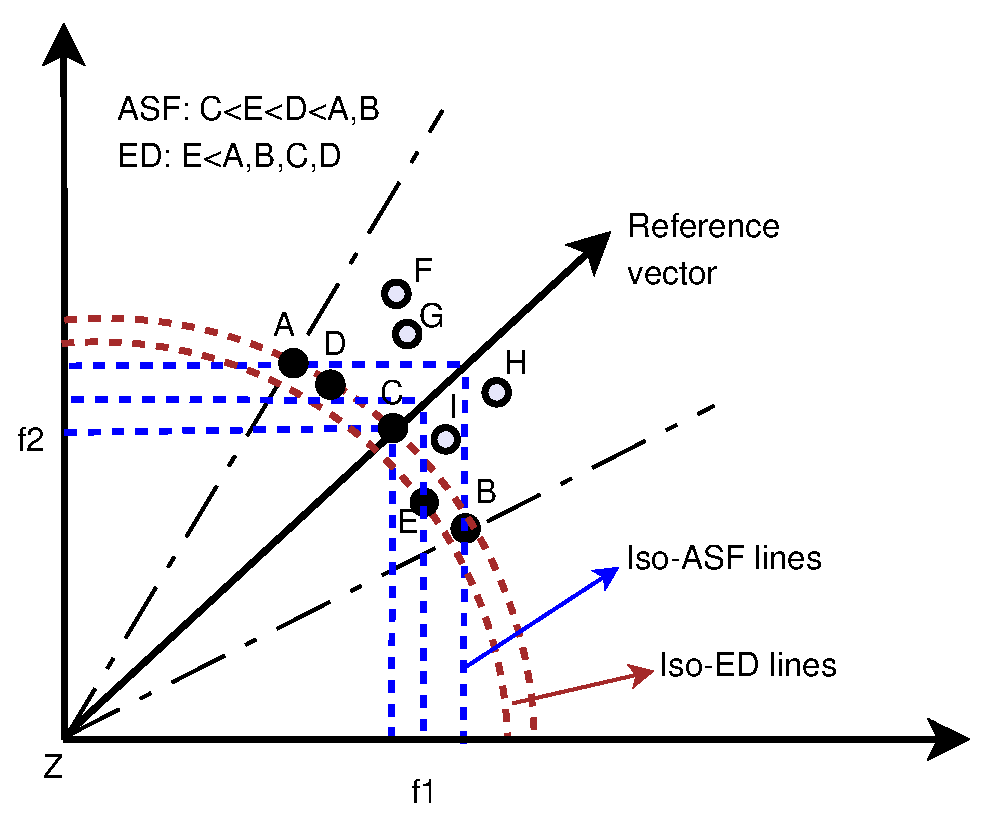
\includegraphics[width = 0.4\textwidth]{figures/asfed.eps}   
	\caption{Schematic comparison of ASF and ED measures}
	\label{fig:compareasfed}
\end{figure}

Additionally, it can also be seen that the formulation of ASF involves a ``max'' function, which makes it more non-linear and difficult to optimize during the local search compared to ED. For example, the active term in ASF will be $i=1$ for the point D, whereas for a slightly improved ASF, the active term will switch to $i=2$. Evidently, as the number of objectives increase, this will cause the active term to switch often between the objectives, making it highly nonlinear and more difficult for a local search algorithm to solve. As a proof-of-concept, consider the local search behavior from 100 solutions constructed using Latin Hypercube Sampling for a 10-objective DTLZ2 problem, shown in Fig.~\ref{fig:asfedls} along a reference vector $\{1/M, 1/M, \ldots, 1/M\}$. For the test problem solutions on the PF should correspond to $G=0$. The average rate of convergence of $G$ though ASF and ED minimization is presented in Fig.~\ref{fig:asfedls}. It is clear that ED, being a much smoother function, is easier to optimize and is therefore more suitable for the local search~(within ``'Identify'' step) discussed in the previous section. On the other hand, to maintain diversity, the ASF-based selection works better, as discussed above. Therefore, overall, this combination~(ASF for selection and ED for local search) is able to provide the best results for most cases in the numerical experiments.     

\begin{figure}[!htb]
	\centering    
	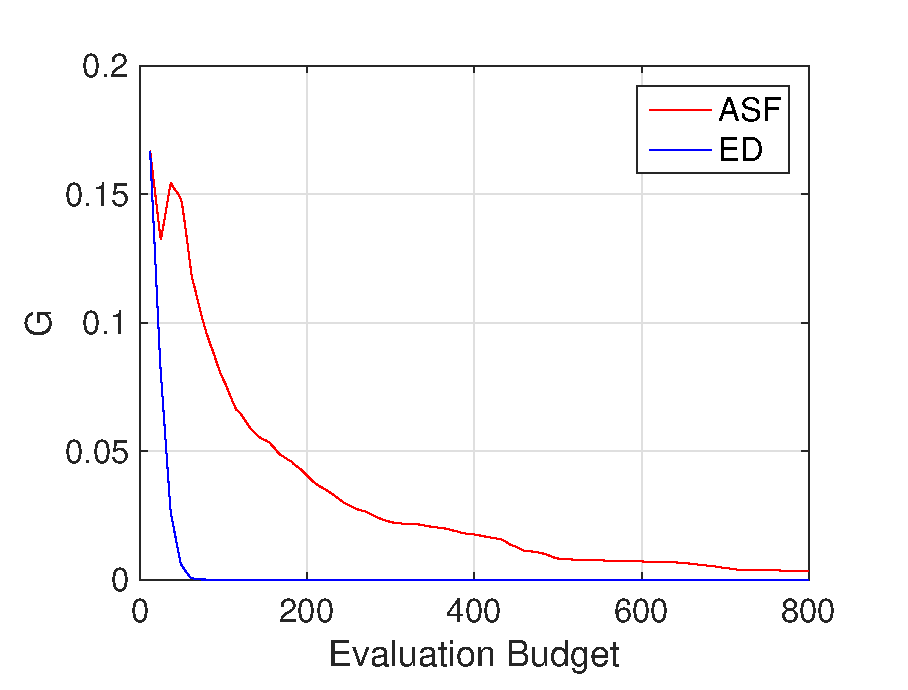
\includegraphics[width = 0.40\textwidth]{figures/dtlz2asfed-10obj.eps}   
	\caption{Local search behavior for ASF and ED measures}
	\label{fig:asfedls}
\end{figure}


\subsubsection{{\color{blue}Vehicle design}}
\label{subsubsec:KHTsubsubsec:3}

Having discussed the performance of the proposed approach on numerical benchmarks, we now present a case study of applying the method to a simulated real-life design problem. For this study, we consider a constrained {\color{blue}vehicle design} problem, originally formulated in \cite{KHTbarnum2010car}. A generic vehicle can be constructed using four modular parts with lengths $L_1$ to $L_4$, heights $H_1$ to $H_4$ and width $W$ as shown schematically in Figure \ref{fig:car}. A slightly modified formulation has been considered here, where we look at midsized vehicles with four doors, forward wheel drive (FWD), and the cargo type for last three part as trunk. The engine is considered to be located in the first part and has a cost denoted by $C_{F3}$. Thus, the ten variables considered for this optimization problem are $\{L_1, L_2, L_3, L_4, W, H_1, H_2, H_3, H_4, C_{F3}\}$. Considering all dimensions in mm, the range of the variables are: $L_1, L_2, L_3, L_4 \in [254,1524], W \in [1676,2032], H_1,H_2,H_3,H_4 \in [914,2032]$ and $C_{F3} \in [600\$,1400\$]$.

\begin{figure}[!htb]
	\centering    
	\subfigure[]{\label{fig:remuwr}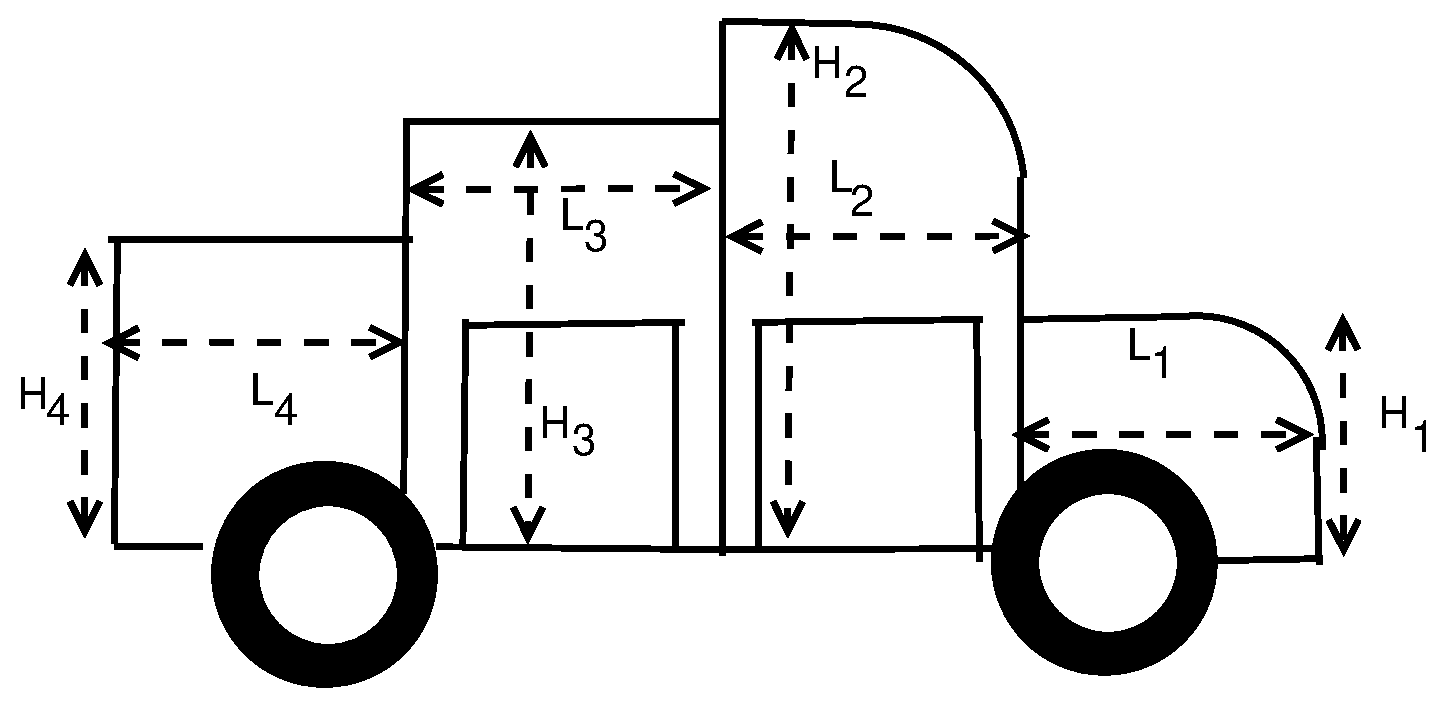
\includegraphics[scale = 0.25]{figures/fig2.eps}}
	\subfigure[]{\label{fig:reducewr}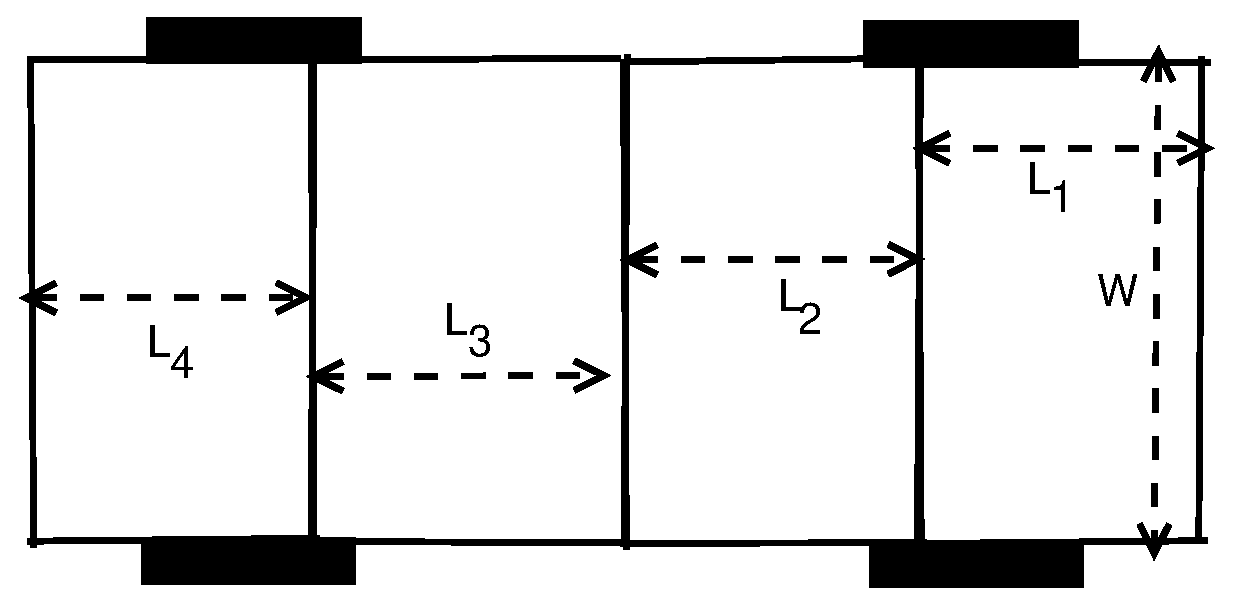
\includegraphics[scale = 0.25]{figures/fig3.eps}}    
	\caption{Vehicle modules: (a) side view, (b) top view}
	\label{fig:car}
\end{figure}

Four different types of engines with different costs are considered: four cylinder ($600 \le C_{F3} \le 800$), V6 ($800 < C_{F3} \le 1000$), V8 ($1000 < C_{F3} \le 1200$) and V8-diesel ($1200 < C_{F3} \le 1400$). Since the first part of the vehicle houses the engine, it is considered to be unavailable for both seating and cargo. The second part is reserved for a seating row. The third parts can allow for either cargo or seating, while the fourth part only allows cargo. For ergonomic feasibility, any part that allows for seating~($L_2$ or $L_3$) must be at least equal to a minimum of  $s_L$ = 1016 mm. If $L_3$ is less than this value, it is automatically assigned for carrying cargo. 

The overall objectives of the problem are to minimize the price, minimize overall weight, maximize towing capacity, maximize cargo space and maximize safety; subject to 17 design constraints. For the sake of numerical experiments to conceptually demonstrate the approach, we consider empirical estimates of each of these objectives as developed in the previous work~\cite{KHTbarnum2010car}, so that the methods could be easily compared and can be further used by the researchers for benchmarking. However, in real-life scenarios, each of these objectives may require intensive numerical calculations~(e.g. crash-simulations, mass integration, field tests, etc.) for more accurate performance estimates, in which case the SaMaO is more suitable for use and could yield the significant advantage. The objectives and constraints are formulated below:  

The price ($f_1$) is defined as:

\begin{equation}\footnotesize
f_1 = m_BC_m + C_t + C_{F2} + C_{F3}
\label{eq:f1}
\end{equation}

where $m_B$ represents the mass of the body, $C_m$ represents the cost of the body material, $C_t$ represents the cost of the tires, $C_{F2}$ represents the cost of the chassis type and $C_{F3}$ represents the cost of the engine type. The value of $C_m$ is taken as 4.41 $\$$/kg, while $m_B$, $C_{F2}$ and $C_t$ are calculated as shown in Eq.~\ref{eq:mb}.

\begin{equation}\footnotesize
\begin{aligned}
m_B & = 0.283*W*\alpha\sum_{i = 1}^4 L_iH_i\\
C_{F2} & = 0.0340 L_f H_2 W C_m\\
C_t & = 20 t_D
\end{aligned}
\label{eq:mb}
\end{equation}

The value of $\alpha$ for first part is 0.003397 whereas the value of $\alpha$ for the parts assigned for seating is considered as 6.834E-04. $L_f$ is the total length of the vehicle~($\sum_{i = 1}^4 L_i$). $t_D$ is the tire diameter, considered to be 584 mm. 

The second objective ($f_2$) is the weight, defined as
\begin{equation}\footnotesize
f_2 = m_B + m_t + m_{F2} + m_{F3},
\label{eq:f2}
\end{equation}

\noindent where $m_t$ is the tire weight, $m_{F2}$ is the weight of the chassis considered as 996.6 kg and $m_{F3}$ is the weight of the engine. $m_t$ is considered as $8 t_D$, whereas $m_{F3}$ proportional to the engine cost, calculated as $0.453C_{F3}$.

The third objective, towing capacity ($f_3$) is expressed as

\begin{equation}\footnotesize
f_3 = -453 \times \sqrt{2(E_f-1)} 
\label{eq:f3}
\end{equation}

\noindent where $E_f$ = 1 for four cylinder, $E_f$ = 2 for V6, $E_f$ = 3 for V8 and $E_f$ = 4 for V8-diesel type engines. Note that the `-' sign above is to convert maximization to minimization problem. Same goes with $f_4$ and $f_5$. 

The fourth objective is the net cargo volume, calculated as shown in Eq.~\ref{eq:f4}. 

\begin{equation}\footnotesize
f_4=\begin{cases}
-0.25(L_2WH_2 + L_3WH_3 + L_4WH_4) & \text{if}~L_2 < s_L, L_3 < s_L\\
-0.25(L_3WH_3 + L_4WH_4) & \text{if}~L_2 \ge s_L, L_3 < s_L\\
-0.25(L_2WH_2 + L_4WH_4) & \text{if}~L_2 < s_L, L_3 \ge s_L\\
-0.25(L_4WH_4) & \text{if}~L_2 \ge s_L, L_3 \ge s_L\\
\end{cases}
\label{eq:f4}
\end{equation}

The fifth objective ($f_5$) reflects the passenger safety, calculated as

\begin{equation}\footnotesize
{\color{blue}f_5=}\begin{cases}
-L_1(loc\_seating - 1) & \text{if}~loc\_seating \neq \emptyset\\
-L_fWH_2 & \text{if}~loc\_seating = \emptyset\\
\end{cases}
\label{eq:f5}
\end{equation}
where $loc\_seating$ is defined as the first seating location, which may be either second or third part. The formulation assumes that the safety will increase if the seating row is further from the front end of the vehicle. 

The constraints for this problem are shown in Eq.~\ref{eq:constr}, and mainly concern the desired limits of each objective, and the practicality of the configuration. 

\begin{equation}\footnotesize
\begin{aligned}
& 0 \$ \le f_1 \le 100000 \$; \quad f_2 \le 22650 kg; \quad f_3 \le 3624 kg \\
& 0.283 m^3 \le f_4 \le 5.66 m^3 \\
& H_2 \ge H_1; \quad H_2 \ge H_3; \quad H_2 \ge H_4; \quad H_3 \ge H_4 \\ 
&L_2 \ge s_L; \quad H_1 \le H_2/2 \\
\end{aligned}
\label{eq:constr}
\end{equation}

To demonstrate the utility of the proposed approach, we compare the performance of SaMaO\textsubscript{ASF-ED} with the same algorithmic framework without surrogates~(denoted simply as MaO). Both algorithms {\color{blue}are run for} a fixed budget $TFE_{max} $of 4000 function evaluations. The population size for MaO and SaMaO is set as 126 ($H$ = 5). {\color{blue}Please take note that for both algorithms, the initial population size is considered as $N_I = 11 \times (n_{var} - 1) = 109$, consistent with the recommendation in \cite{KHTchugh2016krvea}}. 

{\color{blue}To compare the performance, we observe two quantities: (a) the percentage of non-dominated solutions delivered by the two approaches at different stages during the search with respect to the final~(combined) set of non-dominated solutions achieved, and (b) the hypervolume of the obtained approximation till that point in the search. Note that IGD comparison has not been shown for this case since it requires the true PF to be available~(which was the case with the benchmarks but not the case with this problem). The observations are summarized in Fig.~\ref{fig:nd}. It is clear from the plot that SaMaO\textsubscript{ASF-ED} significantly outperforms MaO in terms of both metrics any given stage in the search. At the end of the run~(4000 evaluations), SaMaO is able to deliver nearly four times as many non-dominated solutions as that delivered by MaO, and approximately 15\% better hypervolume than MaO. Moreover, it can be seen that the difference in the performance is substantial right from the beginning. This can be attributed to the fact that with the same population size, both algorithms consume the same evaluations in the first generation; but thereafter SaMaO uses prediction based on the metamodels constructed through these solutions to predict better regions to sample. MaO on the other hand is driven purely by the fitness of the solution, which results in slower convergence and consumption of higher number of evaluations at each generation.  To visualize the solutions at various stages of the search, we observe the matrix plots of the solutions obtained after various numbers of evaluations~(500, 1000, 2000 and 4000). Due to space limitations, these are included in the supplementary material. The inference from the plots is consistent with those from Fig.~\ref{fig:nd}. A much less convergence and diversity of solutions is obtained in general. At the end of the run~(4000 evaluations), both MaO and SaMaO\textsubscript{ASF-ED} were able to find a range of non-dominated solutions with different types of engines, but the number~(and diversity) of non-dominated designs delivered by SaMaO is significantly higher. This is definitely more helpful from the user/designer's point of view as a much wider range of vehicles is available to choose from to closely satisfy particular requirements based on intended usage of the vehicles. At intermediate stages~(e.g. at 500 and 1000 evaluations), the range obtained by MaO did not cover all engine types, whereas that of SaMaO did, clearly reflecting on better diversity off the latter. Therefore, it is evident that with stricter limits on function evaluations, SaMaO\textsubscript{ASF-ED} will be a much more practical approach to obtain diverse, well performing designs quickly. }

\begin{figure}[!htb]
	\centering    
	\subfigure[]{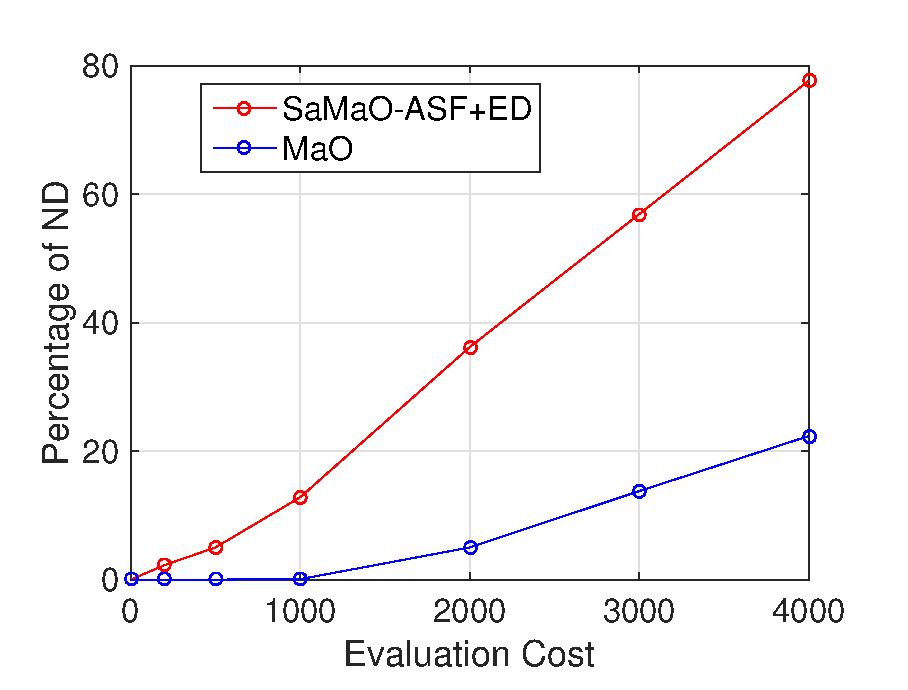
\includegraphics[width = 0.40\textwidth]{figures/fig8.eps}}\\
	\subfigure[]{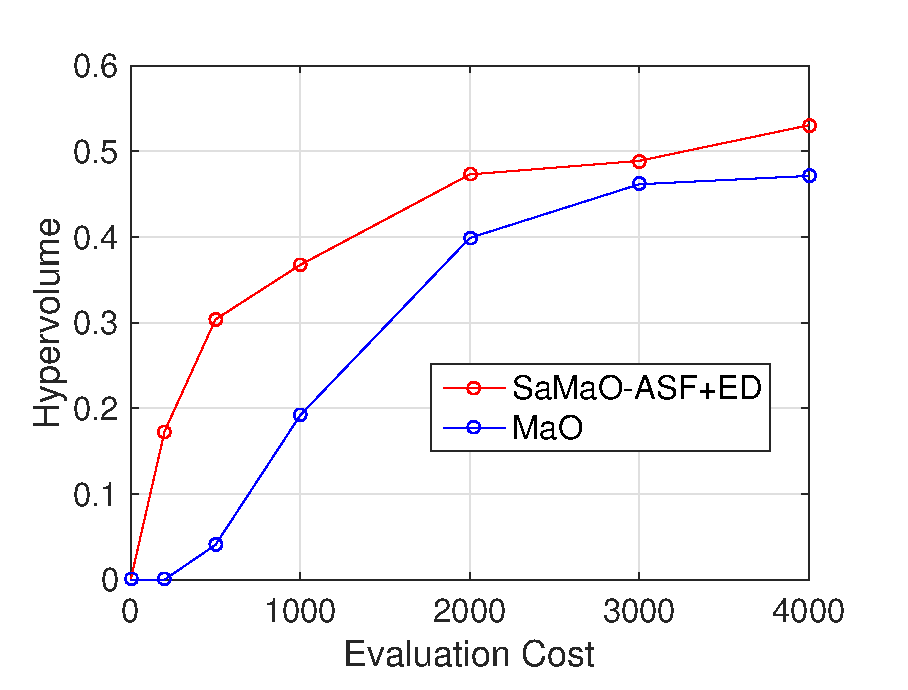
\includegraphics[width = 0.40\textwidth]{figures/fig13.eps}}    
%	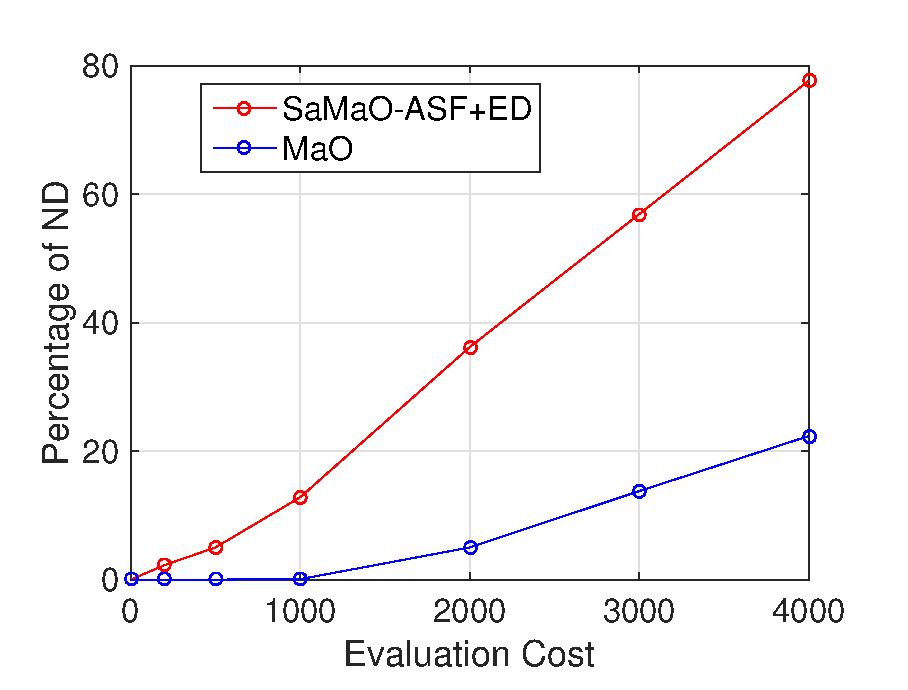
\includegraphics[scale = 0.3]{figures/fig8.eps}   
	\caption{Comparison of MaO and SaMaO\textsubscript{ASF-ED} over function evaluations: (a) fraction of non-dominated solutions (c) Hypervolume}
	\label{fig:nd}
\end{figure}


{\color{blue}
We would like to conclude this section by mentioning some of the limitations of the proposed approach, which will be the subjects of the future extensions of this work. One of the challenges is regarding the handling of large number of \emph{variables} in conjunction with large number of objectives. A possible way to overcome this would be to develop decomposition strategies for both, the objectives and variables and effective ways of interaction between them during the search. Second is that given that this work is predominantly directed towards simulation based optimization, it is important to be able to handle cases where simulations fail, resulting in missing data or numerical divergence. In this regard, the use of ``penalty'' for regions in decision space that result in failed simulations could be one of the possible approach. Lastly, more sophisticated adaptation schemes, can be used to enhance the algorithm further for a variety of irregular fronts, such as inverted, disconnected and degenerated PFs. Recently developed adaptive reference vector schemes such as that in \cite{asaf2017enhanced} could be used towards achieving this goal.  
}


\section{Summary and Conclusions}
\label{sec:KHTsec:5}

In this paper, we introduced a surrogate assisted optimization approach for many-objective optimization. The proposed algorithm relies on principles of decomposition and employs reference vector adaptation in order to deal with Pareto fronts of different shapes. The flexibility of function representation is offered through the use of multiple types of surrogates~(RSM, RBF, Kriging) unlike previous attempts that use a single type of surrogate. Furthermore, it employs adaptive schemes to eliminate need for user defined parameters and rules. To efficiently deal with constrained MaOPs, marginally infeasible solutions are promoted during the early phases of search. In terms of identification of solutions for evaluation at each generation, two different strategies, ASF and ED are compared and contrasted for selection and local search. The performance of the proposed algorithm is objectively evaluated using a range of multi-/many-objective optimization benchmarks with limited computing budget. Thereafter, a case study in {\color{blue}vehicle design} is presented as an application. The numerical experiments and comparisons with the existing approaches clearly highlight the competitive performance of the proposed algorithm and demonstrate its potential for real-life engineering problems involving computationally expensive objectives.  

\scriptsize
\bibliographystyle{asmems4} 
\balance
\bibliography{KHTchapter}


\end{document}
